%\documentclass[handout]{ximera}
\documentclass[nooutcomes]{ximera}

\usepackage{gensymb}
\usepackage{tabularx}
\usepackage{mdframed}
\usepackage{pdfpages}
%\usepackage{chngcntr}

\let\problem\relax
\let\endproblem\relax

\newcommand{\property}[2]{#1#2}




\newtheoremstyle{SlantTheorem}{\topsep}{\fill}%%% space between body and thm
 {\slshape}                      %%% Thm body font
 {}                              %%% Indent amount (empty = no indent)
 {\bfseries\sffamily}            %%% Thm head font
 {}                              %%% Punctuation after thm head
 {3ex}                           %%% Space after thm head
 {\thmname{#1}\thmnumber{ #2}\thmnote{ \bfseries(#3)}} %%% Thm head spec
\theoremstyle{SlantTheorem}
\newtheorem{problem}{Problem}[]

%\counterwithin*{problem}{section}



%%%%%%%%%%%%%%%%%%%%%%%%%%%%Jenny's code%%%%%%%%%%%%%%%%%%%%

%%% Solution environment
%\newenvironment{solution}{
%\ifhandout\setbox0\vbox\bgroup\else
%\begin{trivlist}\item[\hskip \labelsep\small\itshape\bfseries Solution\hspace{2ex}]
%\par\noindent\upshape\small
%\fi}
%{\ifhandout\egroup\else
%\end{trivlist}
%\fi}
%
%
%%% instructorIntro environment
%\ifhandout
%\newenvironment{instructorIntro}[1][false]%
%{%
%\def\givenatend{\boolean{#1}}\ifthenelse{\boolean{#1}}{\begin{trivlist}\item}{\setbox0\vbox\bgroup}{}
%}
%{%
%\ifthenelse{\givenatend}{\end{trivlist}}{\egroup}{}
%}
%\else
%\newenvironment{instructorIntro}[1][false]%
%{%
%  \ifthenelse{\boolean{#1}}{\begin{trivlist}\item[\hskip \labelsep\bfseries Instructor Notes:\hspace{2ex}]}
%{\begin{trivlist}\item[\hskip \labelsep\bfseries Instructor Notes:\hspace{2ex}]}
%{}
%}
%% %% line at the bottom} 
%{\end{trivlist}\par\addvspace{.5ex}\nobreak\noindent\hung} 
%\fi
%
%


\let\instructorNotes\relax
\let\endinstructorNotes\relax
%%% instructorNotes environment
\ifhandout
\newenvironment{instructorNotes}[1][false]%
{%
\def\givenatend{\boolean{#1}}\ifthenelse{\boolean{#1}}{\begin{trivlist}\item}{\setbox0\vbox\bgroup}{}
}
{%
\ifthenelse{\givenatend}{\end{trivlist}}{\egroup}{}
}
\else
\newenvironment{instructorNotes}[1][false]%
{%
  \ifthenelse{\boolean{#1}}{\begin{trivlist}\item[\hskip \labelsep\bfseries {\Large Instructor Notes: \\} \hspace{\textwidth} ]}
{\begin{trivlist}\item[\hskip \labelsep\bfseries {\Large Instructor Notes: \\} \hspace{\textwidth} ]}
{}
}
{\end{trivlist}}
\fi


%% Suggested Timing
\newcommand{\timing}[1]{{\bf Suggested Timing: \hspace{2ex}} #1}




\hypersetup{
    colorlinks=true,       % false: boxed links; true: colored links
    linkcolor=blue,          % color of internal links (change box color with linkbordercolor)
    citecolor=green,        % color of links to bibliography
    filecolor=magenta,      % color of file links
    urlcolor=cyan           % color of external links
}

\title{It's What the Book Says}
\author{Bart Snapp and Brad Findell}

\outcome{Careful definitions of special quadrilaterals and 
the relationships among these shapes.}

\begin{document}
\begin{abstract}
Writing and using careful definitions to describe relationships among special quadrilaterals.  
\end{abstract}
\maketitle


\begin{teachingnote}
The Venn diagram begun below does not help show the relationships among the special quadrilaterals, so a different Venn diagram is needed.  But the main point of the activity is establishing careful definitions of these quadrilaterals.  A secondary point is to compare and contrast the two definitions of trapezoid.  

Here are abbreviated versions of the intended definitions: 
\begin{itemize}\itemsep0em
\item Rectangle:  four right angles (or four congruent angles)
\item Parallelogram:  two pairs of parallel sides
\item Rhombus:  four congruent sides
\item Square:  four right angles and four congruent sides
\item Trapezoid (exclusive): exactly one pair of parallel sides
\item Trapezoid (inclusive): at least one pair of parallel sides
\item Kite: two distinct pairs of adjacent, congruent sides
\end{itemize}

Here are the meta-objectives about the role of definitions:  
\begin{itemize}\itemsep0em
\item Definitions should be precise
\item Definitions should be simple (short and ``minimal'')
\item Additional properties (e.g., opposite sides of a parallelogram are congruent) can be proven from well-chosen definitions 
\item Definitions are ``touchstones'' used to determine whether an object is an example or not
\item Definitions are choices, and different definitions can have different consequences
\end{itemize}

\textbf{Side Note 1:} Both Ohio's standards and the Common Core State Standards allow either definition of trapezoid.  Some textbooks and exams choose one definition.  

\textbf{Side Note 2:} With the inclusive definition of trapezoid, isosceles trapezoid poses an additional challenge:  Should a parallelogram be considered an isosceles trapezoid?  Some textbooks resolve the issue by defining an isosceles trapezoid as a trapezoid with congruent base angles.    

\textbf{Side Note 3:} The above definition of kite excludes rhombuses.  An inclusive definition is worth exploring if there is time.  

\end{teachingnote}

\begin{problem}
Do the following task fifth-grade task: Put the
terms \textbf{square}, \textbf{rhombus}, and \textbf{parallelogram} in
the Venn diagram below.  
\begin{image}
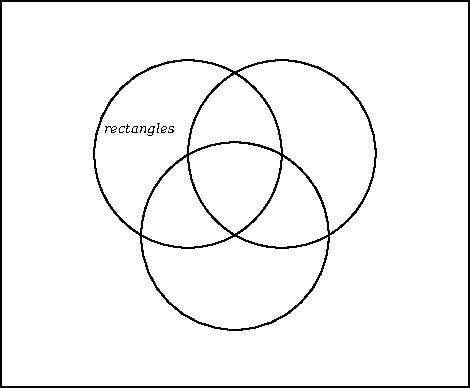
\includegraphics{venn1.pdf}
\end{image}
\end{problem}

\begin{problem} 
Critique the task above based on mathematical content.
\end{problem}

\newpage 
\begin{problem}
Supposing we know that a quadrilateral is a polygon with four sides, write clear and succinct definitions of each of the following terms: 
\begin{enumerate}
\itemsep18pt
\item A \textit{rectangle} is a quadrilateral 
\item A \textit{parallelogram} is a quadrilateral
\item A \textit{rhombus} is a quadrilateral
\item A \textit{square} is a quadrilateral
\item A \textit{trapezoid} is a quadrilateral
\item A \textit{kite} is a quadrilateral
\end{enumerate}
\end{problem}
\bigskip

\begin{problem} 
Create a Venn diagram showing the correct relationships
among these quadrilaterals. Be ready to present and defend your
diagram to your peers.
\end{problem}

\end{document}
